\section{Working Principles}
\label{sec:working_principles}

\subsection{Commercial atomic clocks}
\label{sub:commercial_atomic_clocks}

We use the alkaline metal to use the single valence electron that exhibit a microwave transition (microwave frequency $300MHz \rightarrow 300GHz$).
Because of this, we have the following properties:

\begin{itemize}
    \item Ground state hyperfine splitting of the order of $~GHz$ so that we can use RF electronics.
    \item Simple electronic structure that allow a large optical absorption and possible use of optical detection.
\end{itemize}

\paragraph{Double optical-microwave resonance}

\textbf{Every things happens on the reference cell rubidium inside the microwave cavity.}

This is the technique used in the Rubidium atomic clock (table scale at least).

Here we have a first discharge lamp that excites the $Rb^{87}$ atoms.
In particular, we are here working between the $5^2S_{1/2}$ and the $5^2P$ fine states.
The $5^2S_{1/2}$ state is split into two hyperfine states, $F=1$ and $F=2$ (where 1 indicate the lower of the two hyperfine states).
From the initial situation, we want to move every electron to the $F=2$ state.
To do so, we use a first lamp that emit exactly at the energy difference between the $5^2P$ and the $5^2S_{1/2}$ states.
This is a circularly polarized photo $\sigma^+$, and it will induce a population inversion between the two hyperfine states, so that we have more atoms in the $F=2$ state.

% Once we are shure the population inversion is done, we can also going through a $Rb^{85}$ filter that

Once we have the population inversion, we can go through a microwave cavity that will induce a transition between the two hyperfine states.
In particular, our aim is to have a wave that is exactly at the frequency of the transition between the two hyperfine states of the $5^2S_{1/2}$ fine state.
If we succeed, we will have a resonance, and all the electrons will switch back to the $F=1$ state (ground state).
By doing so, we end up with basically the starting situation and our initial beam of circularly polarized light will be absorbed again by the atoms.

If this happens, than if we use a photodetector that give us a signal of how much light is absorbed, we will have a peak in the signal when the microwave frequency is exactly the one of the transition between the two hyperfine states.
Or similarly, a dip if we use a photodetector that give us a signal of how much light is transmitted (it's absorbed at that frequency).

\begin{figure}[H]
    \centering
    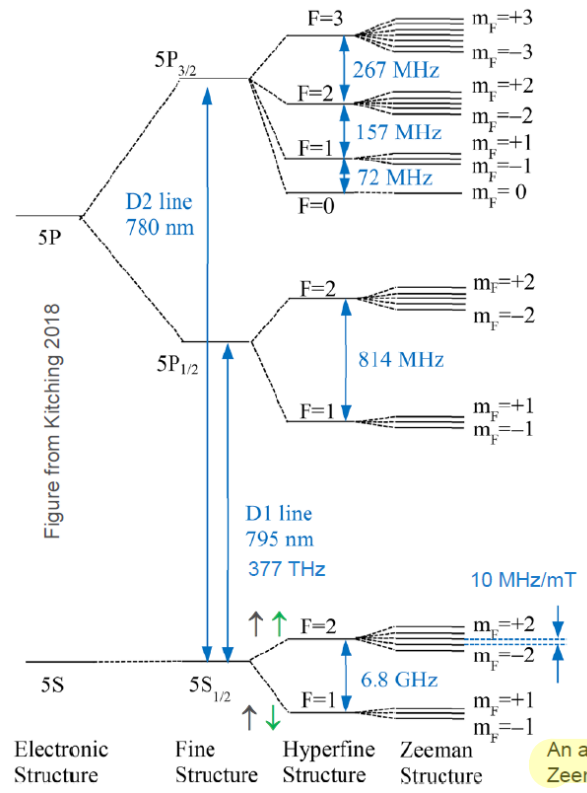
\includegraphics[width=\linewidth]{img/02.1-rubidium-electronic-structure}
    \caption{Rubidium 87 electronic structure (external energy levels)}
    \label{fig:rubidium-electronic-structure}
\end{figure}

\paragraph{More in depth}

Dipole transition selection rules:
\begin{itemize}
    \item Excitation by a circularly polarized light $\sigma^+$: $\Delta m_f = +1$
    \item Spontaneous emission: $\Delta m_f = 0, \pm 1$, but on average $\Delta m_f = 0$
\end{itemize}

In the end, we are sure that pumping will force population inversion generating excess in the $F=2$ state.

The microwave cavity on the other hand (if in complete resonance with the transition between the two hyperfine states) will induce a transition so that the population will be inverted again.

This result in the possibility for the reference cell to absorb again the circularly polarized light, and the trasmissibility of the light will be at a minimum.

\paragraph{Filter cell of $Rb^{85}$}

Since as pumping device we use a rubidium lamp, we will have both the photons coming from the $5^2P \rightarrow 5^2S_{1/2} F=1$ (the one that we are interested in) and the photons coming from the $5^2P \rightarrow 5^2S_{1/2} F=2$ (the one that we want to avoid since their effect is the one that must be provided by the microwave cavity).

To eliminate those photons, we add a filter cell of $Rb^{85}$ that will absorb the photons coming from the $5^2P \rightarrow 5^2S_{1/2} F=2$ transition given that the energy difference between the two its transitions $5^2P \rightarrow 5^2S_{1/2} F=3$ is almost exactly the same as the one of the $5^2P \rightarrow 5^2S_{1/2} F=2$ transition of $Rb^{87}$.
Ate the same time, $Rb^{85}$ will not absorb the photons coming from the $5^2P \rightarrow 5^2S_{1/2} F=1$ transition of $Rb^{87}$.

\begin{figure}[H]
    \centering
    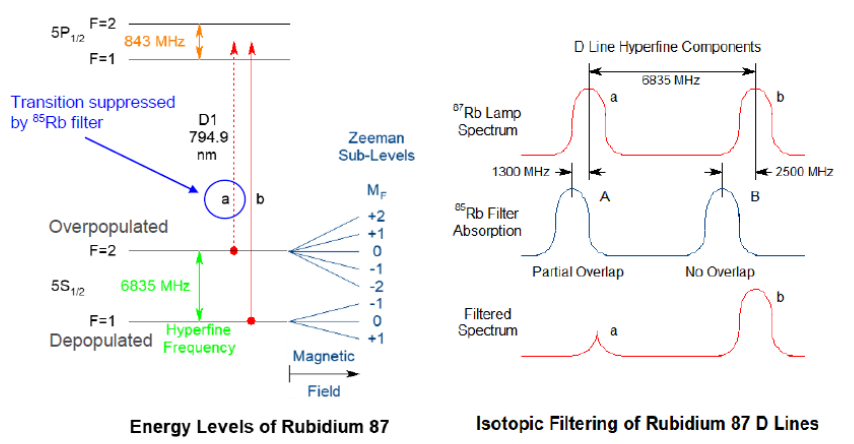
\includegraphics[width=\linewidth]{img/02.2-overlap-for-filtering-rubidium}
    \caption{Overlap of the two transitions of $Rb^{85}$ and $Rb^{87}$}
    \label{fig:overlap-for-filtering-rubidium}
\end{figure}

\paragraph{Cesium atomic clock}

For the cesium atomic clock unfortunately we cannot use the same technique.
So in the end, the option is only to use a different source for the light, and in particular a very stable and accurate single-mode narrow-linewidth laser.
In the end, this approach is less reliable than the combination of the $Rb^{87}$ lamp and the $Rb^{85}$ filter.

\paragraph{Problem so far with the double resonance approach - Power consumption}

All components described so far has to be kept at a constant temperature and pressure to avoid any shift in the frequency of the transition.
This means that our system must include stabilization in temperature driven by a oven controlled sensor and heater.
The power consumption of this system is distributed as follows:

\begin{itemize}
    \item $10\%$: Lamp Exciter
    \item $10\%$: RF Excitation
    \item $10\%$: Electronics
    \item $70\%$: Thermal stabilization oven
\end{itemize}

It's clear how the oven and the thermal stability is the most power consuming part of the entire system.

\paragraph{Problem so far with the double resonance approach - Size}

Another problem is given by the minimum theoretical size of the system.
The RF cavity must be at least half the wavelength of the microwave frequency.
This means that for a microwave frequency of $6.8GHz$ we need a cavity of at least $L_{min} = \frac{\lambda}{2} = \frac{c}{2f} = \frac{3 \cdot 10^8}{2 \cdot 6.8 \cdot 10^9} = 22mm$.

\paragraph{Problem so far with the double resonance approach - Stark shift}

Because of possible electric field, the energy levels of the atoms can be shifted (broadened).
This means that even if our microwave frequency is exactly the one of the transition, the energy levels of the atoms can be shifted so that the resonance is not perfect and the absorption of the light is not at a minimum.
Basically, the position of the dip in the transmissivity is shifted.

\subsection{CSAC - Chip Scale Atomic Clock}

\paragraph{Coherent population trapping (CPT)}

CPT is based on the principle of trapping the population of the atoms in a coherent superposition of the ground states.

We are now interest in apply exactly the energy level corresponding to $\frac{5^2S_{1/2} F=1 + 5^2P_{3/2} F=2}{2}$.
If we succeed in apply this energy level, we will have that our electron will most probably finish in the middle of the two hyperfine states.
This will cause the atom to be impossibilities to absorb the light because of destructive interference between the ac and bc transition probability amplitudes.
Given so, if we observe the spectrum of the light transmitted through the atoms, we will have a peak in the transmissivity at the frequency of the transition (where the CPT happens, and the atoms are not absorbing the light).

If our system is based on Rubidium as the principal element, then our target in frequency of the oscillator is $6.8/2 GHz = 3.4 GHz$, while if our system is based on Cesium, then our target in frequency of the oscillator is $9.2/2 GHz = 4.6 GHz$.

CPT is visible from a transmissivity(frequency) plot like in Figure \ref{fig:CPT-transmissivity-frequency}.

\begin{figure}[H]
    \centering
    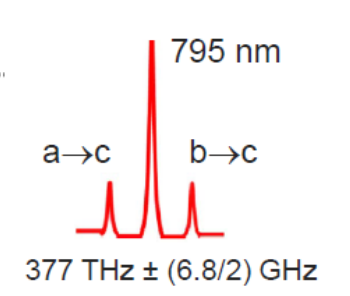
\includegraphics[width=\linewidth]{img/02.3-CPT-transmissivity-frequency}
    \caption{Transmissivity(frequency) plot of a CPT system}
    \label{fig:CPT-transmissivity-frequency}
\end{figure}

\paragraph{Benefits of CPT over double resonance}

By using the CPT technique, we can avoid the use of the microwave cavity and the filter cell of $Rb^{85}$.
This means that we can avoid the power consumption of the oven and the thermal stabilization, and we can avoid the size of the microwave cavity.
In the end, we can have a system that is much smaller and with a much lower power consumption.

The only problem here is that our system must be able to generate a very stable and accurate single-mode narrow-linewidth laser.
The less precise the laser, the less precise the peak in the transmissivity plot (and possible shifted to the wrong frequency).
However, once we have the laser, we can also think of using more than one just element.
In fact, we should opt to pick an element with higher frequency of the transition, so that we can have a more precise peak in the transmissivity plot (as Cesium for example).

Here follows the two systems.

\begin{figure}[H]
    \centering
    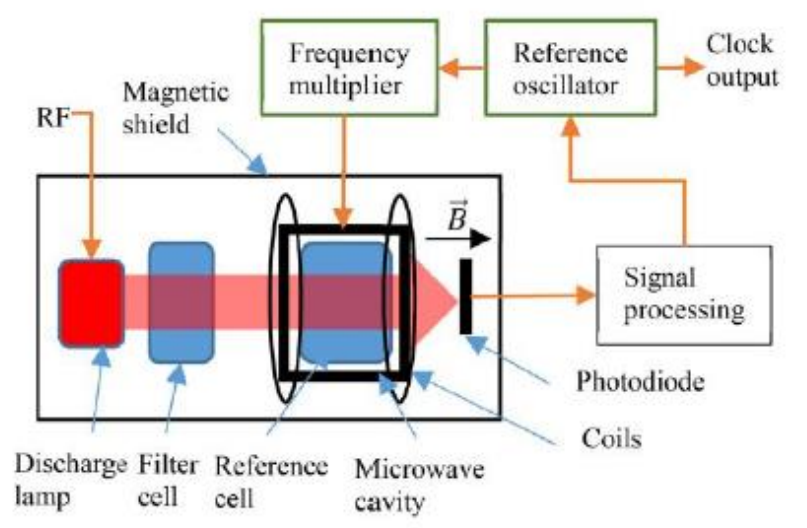
\includegraphics[width=\linewidth]{img/02.4-double-resonance-system}
    \caption{Double resonance system}
    \label{fig:double-resonance-system}
\end{figure}

\begin{figure}[H]
    \centering
    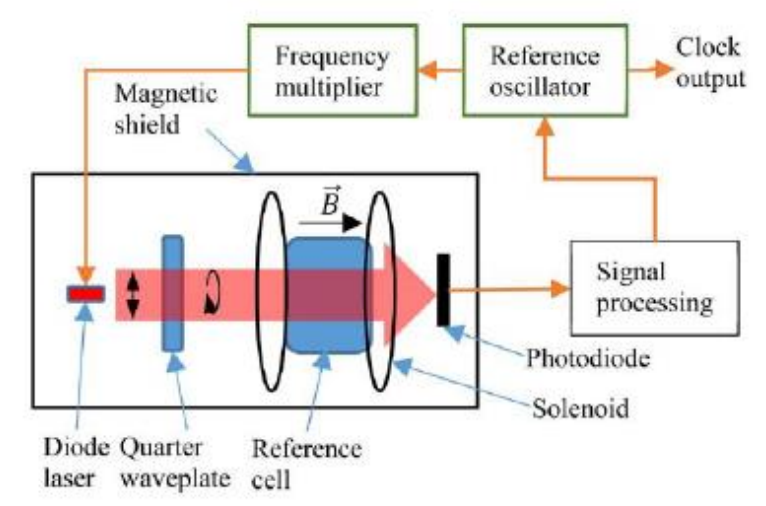
\includegraphics[width=\linewidth]{img/02.5-CPT}
    \caption{CPT}
    \label{fig:CPT}
\end{figure}

% \paragraph{VCSEL - Vertical Cavity Surface Emitting Laser}

\paragraph{Role of buffer gas mixture}

The buffer gas mixture is used to increase the lifetime of the atoms in the excited state.